\documentclass[tikz,border=10pt]{standalone}
\usepackage[utf8]{inputenc}
\usepackage[T1]{fontenc}
\usepackage[english]{babel}
\usepackage{graphicx}
\usepackage{amsmath,amssymb}
\usepackage{tikz}
\usepackage{hyperref}
\usepackage{geometry}
\usepackage{fancyhdr}
\usepackage{listings}
\usepackage{color}
\usepackage{caption}
\usepackage{booktabs}
\usepackage{longtable}
\usepackage{float}
\usepackage{array}
\usepackage{subfigure}
\usepackage{multirow}
\usepackage{multicol}
\usepackage[acronym]{glossaries}
\usepackage{xcolor}
\usetikzlibrary{shapes.geometric,arrows,positioning,calc,fit}

\begin{document}
\pagecolor{white}
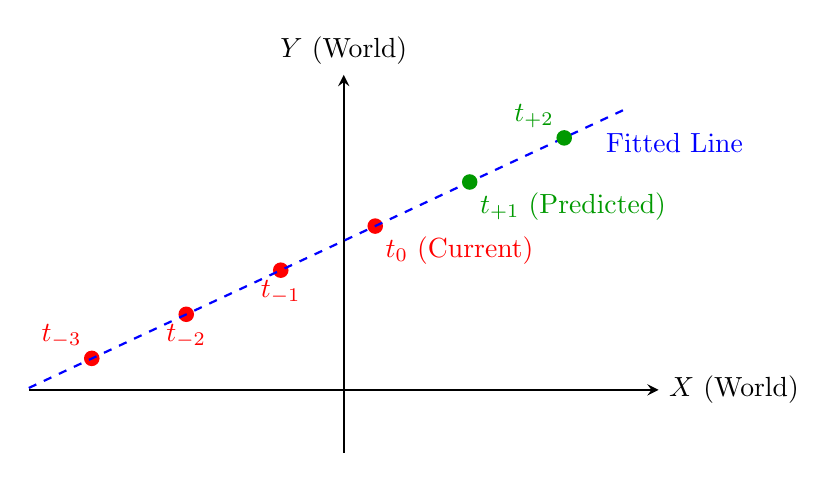
\begin{tikzpicture}[>=stealth, scale=0.8, thick]
    % Draw grid / axes
    \draw[->] (-5,0) -- (5,0) node[right] {$X$ (World)};
    \draw[->] (0,-1) -- (0,5) node[above] {$Y$ (World)};
    
    % Draw historical points (crosses/dots)
    \filldraw[red] (-4, 0.5) circle (3pt) node[above left] {$t_{-3}$};
    \filldraw[red] (-2.5, 1.2) circle (3pt) node[below] {$t_{-2}$};
    \filldraw[red] (-1.0, 1.9) circle (3pt) node[below] {$t_{-1}$};
    \filldraw[red] (0.5, 2.6) circle (3pt) node[below right] {$t_{0}$ (Current)};
    
    % Draw regression line
    \draw[blue, thick, dashed] (-5, 0.03) -- (4.5, 4.47);
    \node[blue, below right] at (4.0, 4.23) {Fitted Line};
    
    % Draw future prediction points
    \filldraw[green!60!black] (2.0, 3.3) circle (3pt) node[below right] {$t_{+1}$ (Predicted)};
    \filldraw[green!60!black] (3.5, 4.0) circle (3pt) node[above left] {$t_{+2}$};
\end{tikzpicture}
\end{document}